\documentclass[24pt,pdf,hyperref={unicode},aspectratio=169]{beamer}
\usepackage[utf8]{inputenc}
\usepackage[russian]{babel}
\usepackage{tikz}
\begin{document}

\tikzstyle{dedge} = [draw,thick,->]
\tikzstyle{edge} = [draw,thick,-]
\tikzstyle{ver} = [circle, draw=black]


\begin{frame}\frametitle{Ориентированный граф (орграф)}
\uncover<+->{$$
G=(V,E)
$$}
\uncover<+->{$$
E\subset V\times V
$$}
\uncover<+->{$$
V=\{2,3,4,6,8\}
$$}
\uncover<+->{$$
E=\{(4,2),(6,2),(6,3),(8,2),(8,4)\}=\{(a,b)\ :\ a\in V,\ b\in V,\ a\%b = 0\}
$$}

\uncover<+->{
\begin{center}
\begin{tikzpicture}[x=2cm,y=-2cm]
\node[ver](n2) at (0,0) {2};
\node[ver](n3) at (1,0) {3};
\node[ver](n4) at (0,1) {4};
\node[ver](n6) at (1,1) {6};
\node[ver](n8) at (-1,1) {8};
\path[dedge] (n4) -- (n2);
\path[dedge] (n6) -- (n2);
\path[dedge] (n6) -- (n3);
\path[dedge] (n8) -- (n2);
\path[dedge] (n8) -- (n4);


\end{tikzpicture}
\end{center}
}
\end{frame}

\begin{frame}\frametitle{Неориентированный граф}

\uncover<+->{$$
G=(V,E)
$$}
\uncover<+->{$$
E=\{\ \{a,b\}\ :\ a,b\in V \}
$$}
\uncover<+->{$$
V=\{1,2,3,4,5\}
$$}
\uncover<+->{$$
E=\{(1,3),(1,5), (3,5), (2,4) \}=\{(a,b)\ :\ a\in V,\ b\in V,\ (a+b)\% 2 = 0 \}
$$}

\uncover<+->{
\begin{center}
\begin{tikzpicture}[x=2cm,y=-2cm]
\node[ver](n1) at (0,0) {1};
\node[ver](n2) at (1,0) {2};
\node[ver](n3) at (0,1) {3};
\node[ver](n5) at (1,1) {5};
\node[ver](n4) at (2,1) {4};
\path[edge] (n2) -- (n4);
\path[edge] (n1) -- (n3);
\path[edge] (n3) -- (n5);
\path[edge] (n1) -- (n5);

\end{tikzpicture}
\end{center}
}

\end{frame}

\begin{frame}
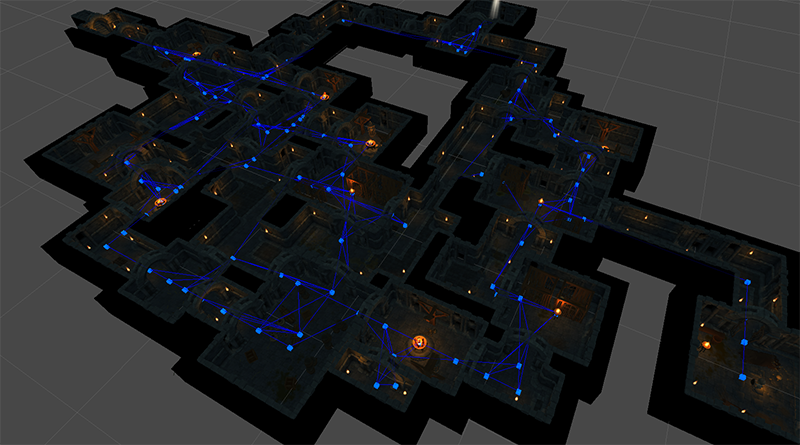
\includegraphics[width=\textwidth]{waypoints.png}
\end{frame}

\begin{frame}
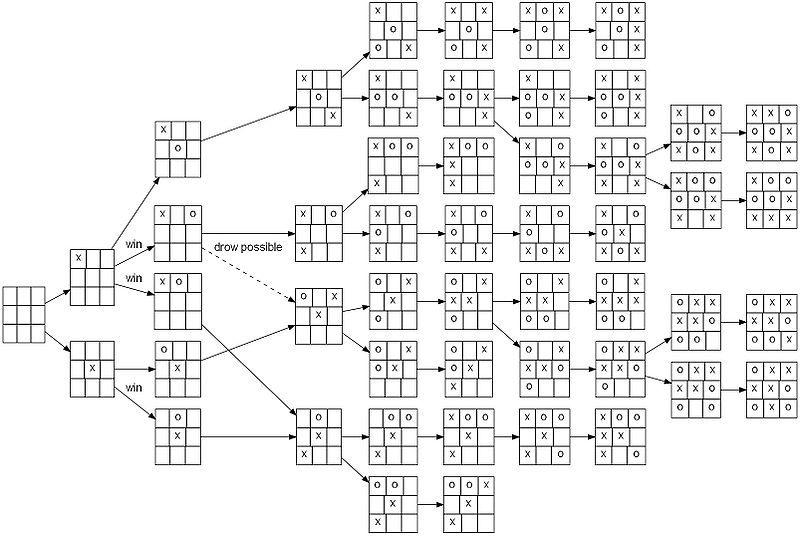
\includegraphics[height=\textheight]{tictactoe.jpg}
\end{frame}

\begin{frame}
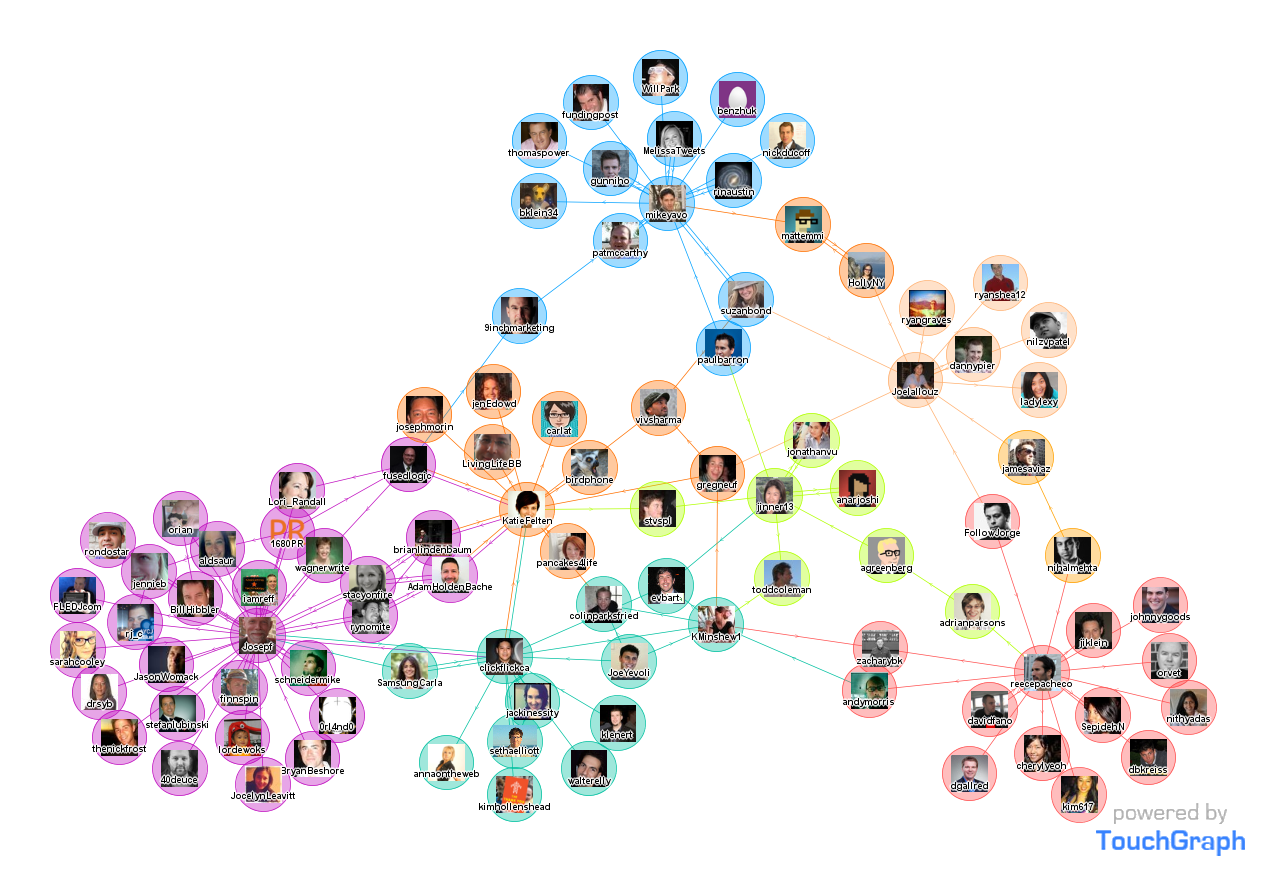
\includegraphics[height=\textheight]{socnetwork.png}
\end{frame}

\begin{frame}

\uncover<+->{
Ребро $e$ {\bf инцидентно} вершине $v$, если $e=(v,w)$ или $e=(w,v)$ для некоторого $w$
}\\[0.3cm]

\uncover<+->{
Вершины $v$ и $w$ {\bf индицентны}, если $(v,w)\in E$.
}\\[0.3cm]

\uncover<+->{
{\bf Степенью вершины} в неориентированном графе называют количество инцидентных ей ребер. Для ориентированных графов разделяют степень захода и степень исхода.
}\\[0.3cm]

\uncover<+->{
{\bf Путь (маршрут)} -- это последовательность $v_1,e_1,v_2,e_2,\ldots,v_n$, где $e_i=(v_i,v_j)$, $e_i\in E$, $v_i\in V$.
}\\[0.3cm]

\uncover<+->{
{\bf Простой путь} -- это путь, в котором все ребра и вершины различны.
}\\[0.3cm]

\uncover<+->{
{\bf Цикл (контур)} -- это путь, в котором первая и последняя вершина совпадают, но других совпадений нет.
}\\[0.3cm]

\uncover<+->{
Неориентированный граф {\bf связен}, если между любыми двумя его вершинами существует путь. Для орграфов такое условие называют {\bf сильной связностью}. {\bf Слабая связность} орграфа означает связность соответствующего ему неориентированного графа.
}
\end{frame}

\begin{frame}
\uncover<+->{
{\bf Дерево} -- это связный неориентированный граф, не содержащий циклов.
}\\[0.5cm]


\uncover<+->{
\begin{center}
\begin{tikzpicture}[x=1cm, y=-1cm]
\node[ver] (n1) at (0,0) {};
\node[ver] (n2) at (-1,1){};
\node[ver] (n3) at (1,1){};
\node[ver] (n4) at (0,1){};
\node[ver] (n5) at (0,2){};
\node[ver] (n6) at (2,2){};
\path[edge] (n1) -- (n2);
\path[edge] (n1) -- (n3);
\path[edge] (n1) -- (n4);
\path[edge] (n3) -- (n5);
\path[edge] (n3) -- (n6);
\end{tikzpicture}
\end{center}
}

\uncover<+->{
{\bf Лист} -- это вершина дерева, имеющая степень 1.
}\\[0.5cm]

\uncover<+->{
{\bf Корень} -- это произвольно выбранная и зафиксированная вершина дерева.
}\\[0.5cm]

\uncover<+->{
Несвязный неориентированный ациклический граф иногда называют {\bf лесом}.
}

\end{frame}

\begin{frame}

\begin{center}
\begin{tikzpicture}[x=2cm, y=-2cm]
\node[ver] (n1) at (0,0)  {0};
\node[ver] (n2) at (-1,1)  {1};
\node[ver] (n3) at (1,1)  {2};
\node[ver] (n4) at (-1,2){3};
\node[ver] (n5) at (1,2) {4};

\path[edge] (n1)--(n2);
\path[edge] (n1)--(n3);
\path[edge] (n2)--(n4);
\path[edge] (n2)--(n5);
\path[edge] (n3)--(n4);
\path[edge] (n3)--(n5);

\end{tikzpicture}
\end{center}

\end{frame}


\begin{frame}

\begin{columns}
\column{0.5\textwidth}
\begin{center}
\begin{tikzpicture}[x=2cm,y=-2cm]

\node[ver] (n0) at (0,0) {0};
\node[ver] (n1) at (1,1) {1};
\node[ver] (n2) at (-1,1.5) {2};
\node[ver] (n3) at (1,2) {3};
\node[ver] (n4) at (0,3) {4};

\path[dedge] (n0) -- (n1);
\path[dedge] (n0) -- (n2);
\path[dedge] (n1) -- (n2);
\path[dedge] (n1) -- (n3);
\path[dedge] (n2) -- (n3);
\path[dedge] (n2) -- (n4);
\path[dedge] (n3) -- (n4);


\end{tikzpicture}
\end{center}
\column{0.5\textwidth}

\begin{center}
\begin{tikzpicture}[x=2cm,y=-2cm]

\node[ver] (n0) at (0,0) {0};
\node[ver] (n1) at (0,1) {1};
\node[ver] (n2) at (1,2) {2};
\node[ver] (n3) at (-1,2) {3};
\node[ver] (n4) at (0,3) {4};

\path[dedge] (n0) -- (n1);
\path[dedge] (n1) -- (n2);
\path[dedge] (n2) -- (n3);
\path[dedge] (n3) -- (n1);
\path[dedge] (n2) -- (n4);
\path[dedge] (n3) -- (n4);

\end{tikzpicture}
\end{center}
\end{columns}
\end{frame}

\begin{frame}

\uncover<+->{{\bf Лемма 1. Если в орграфе есть циклы, он не может быть топологически отсортирован.}}\\[0.1cm]

\uncover<+->{ Из любой вершины цикла есть путь в любую другую, а значит, в каком бы порядке мы их не расположили, этот порядок не будет топологической сортировкой}\\[0.3cm]

\uncover<+->{{\bf Лемма 2. Если в орграфе нет циклов, то в нем есть вершина с нулевой степенью захода.}}\\[0.1cm]

\uncover<+->{От противного: пусть такой вершины нет, значит, для каждой вершины есть входящее в нее ребро. Возьмем любую $v_0$, затем $v_1$ такую, что ребро из $v_1$ ведет в $v_0$, и так далее. Эту последовательность можно продолжить бесконечно, но вершин в графе -- конечное число, следовательно, вершины повторятся, и образуют цикл.}


\end{frame}

\begin{frame}

\uncover<+->{{\bf Лемма 3. Если в орграфе нет циклов, он может быть топологически отсортирован}}\\[0.1cm]

\uncover<+->{
База индукции: очевидно для двухэлементного орграфа.

Шаг индукции. По Лемме 2, есть вершина $u$ с нулевой степенью захода. Исключим вершину $u$ из графа со всеми исходящими ребрами. По предположению индукции, в получившемся графе есть топологическая сортировка $v_1,\ldots,v_n$. Тогда $u,v_1,\ldots,v_n$ будет топологической сортировкой исходного графа: в $u$ нет входящих ребер, а значит, нет и пути из вершин $v_1,\ldots,v_n$.}

\end{frame}

\end{document}